\documentclass[a4paper,11pt]{article}
\usepackage[left=1.5cm, right=1.5cm, top=2cm, bottom=1cm]{geometry}
\usepackage{graphicx}
\usepackage{amssymb}
\usepackage{amsmath}
\usepackage{wrapfig}

\begin{document}
\title{\LARGE{\textbf{ECEN 204 Lab 5}\\BJT Applications}}
\author{Niels Clayton : 300437590\\ \textbf{Lab Partner: }Nickolai Wolfe}
\date{September 22, 2019}
\maketitle
\hrule

\section{BJT as a switch}
\begin{figure}[h]
 \begin{center}
  \fbox{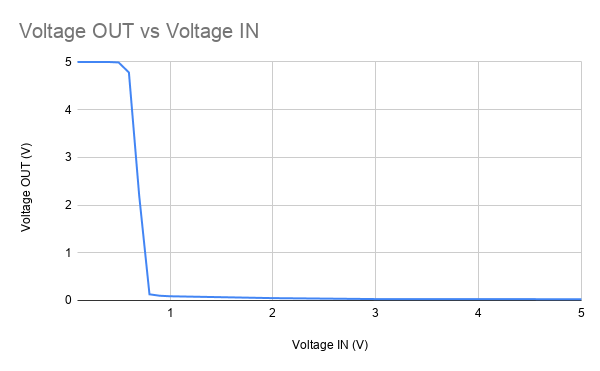
\includegraphics[width = 0.8\textwidth]{switch.png}}
  \vspace{-8pt}
  \caption{Base voltage in vs collector voltage out}
 \end{center}
\end{figure}

It can be seen in figure 1 that when the voltage into the base of the transistor ($V_B$) is below 0.7V, the BJT is not considered to be operating, and when $V_B$ is larger than 0.7V the BJT is considered to be operating. Because of this, when $V_B < 0.7V$ there is a large voltage difference between the collector and the emitter due to the BJT not being active and having near infinite resistance, This can be considered a logical HIGH. When $V_B > 0.7V$ there is little to no voltage difference between the collector and the emitter, which can be seen as a logical LOW. From this the following logic table can be constructed, simulating a logical NOT operation.

\begin{center}
\begin{tabular}{|c|c|}  
\hline
 IN & OUT\\
\hline
LO & HI \\
HI & LO\\
\hline
\end{tabular}
\end{center}
\pagebreak

\begin{figure}[h]
 \begin{center}
  \fbox{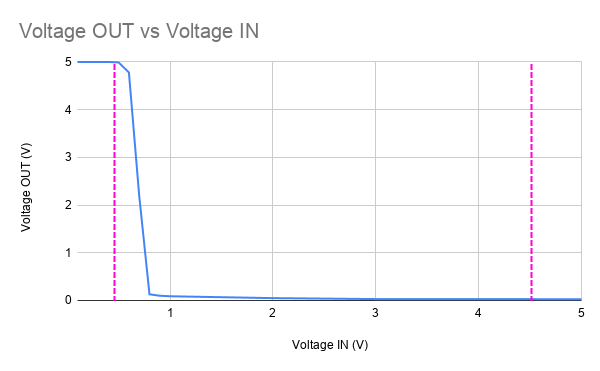
\includegraphics[width=0.5\textwidth]{switch_load.png}
		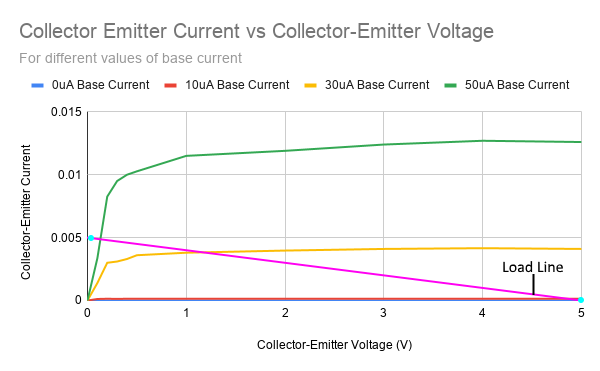
\includegraphics[width=0.5\textwidth]{load_first.png}}
  \caption{On the  left, the input-output voltage characteristics of a BJT, On the right the load-line of the BJT with Q-points marked}
 \end{center}
\end{figure}

In the first image in figure 2, the collector emitter voltages are taken at different base voltages (0.4V for LO and 4.5V for HI). These then give corresponding outputs of $\approx$ 5V for LO input, and $\approx$ 0V for HI input.

On the second image, the load-line was then plotted by taking a line between the short-circuit voltage of 5V, and the open-circuit current of 0.005mA. the Q-points were then plotted by marking the outputs of $\approx$ 5V for LO, and $\approx$ 0V for HI on the curve.

from this, it can be seen that for an input voltage of LO, the Q-point will be located within the cut-off region of the transistor characteristic curve, and when the input is HI, the Q-point is located within the saturation region of the curve. 

From figure two it can also be seen that for an input voltage of 2.5V, the output voltage of the BJT will be $\approx$ 5V, leading to a logical HI.

\section{Value of $\beta$ in the active region}

\begin{center}
\begin{tabular}{|c|c|c|c|}  
\hline
 $ I_B$  & $V_{CE}$ (V) & $I_C$ & $\beta$\\
\hline
0uA & 4 & 0.7uA & NaN\\
10uA & 1 & 0.14mA & 14\\
10uA & 4 & 0.14mA & 14\\
30uA & 1 & 3.8mA & 126.7\\
30uA & 4 & 4.15mA & 138.7\\
50uA & 1 & 11.5mA & 230\\
50uA & 4 & 12.7mA & 254\\
\hline
\end{tabular}
\end{center}

From the above table it can be seen that as the current into the base of the transistor increases, the beta value will increase dramatically, however once $V_{CE}$ is achieved to saturate the current through the transistor, there will be very little gain in the $\beta$ value by raising the voltage.

\begin{center}
\begin{tabular}{|c|c|c|c|}  
\hline
Measurement & $\beta$ average & $\beta$ maximum & $\beta$ minimum\\
\hline
Own & 129 & 254 & 14\\
\hline
Another 1 & & & \\
\hline
Another 2 & & & \\
\hline
Another 3 & & & \\
\hline
\end{tabular}
\end{center}

From this table it can be seen that the use of $\beta$ for calculations would not be advised as the $\beta$ value can vary wildly from one transistor to another, as well as  varying based on the voltages and currents applied to the transistor.

\pagebreak
\subsection{Calculation of $V_{CE}$ \& $I_C$ with varying $\beta$ }

\section{BJT as a switch}
\begin{figure}[h]
 \begin{center}
  \fbox{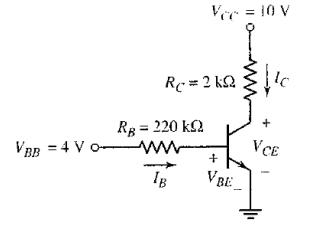
\includegraphics[width = 0.7\textwidth]{beta.jpg}}
  \vspace{-8pt}
  \caption{example circuit for $\beta$ calculations}
 \end{center}
\end{figure}

$$ I_B = \dfrac{V_{BB} - V_{BE}}{R_B} = \dfrac{4-0.7}{220k} = 15uA  $$
$$ I_C = \beta I_B  $$
For $\beta$ = 14:  $$I_C = 0.21mA$$
For $\beta$ = 254:  $$I_C = 3.81mA$$
$$ V_{CE} = V_{CC} - I_C R_C $$
For $\beta$ = 14:  $$V_{CE} = 9.58$$
For $\beta$ = 254:  $$V_{CE} = 2.38$$
\pagebreak

\section{BJT as an amplifier}


\begin{figure}[h]
 \begin{center}
  \fbox{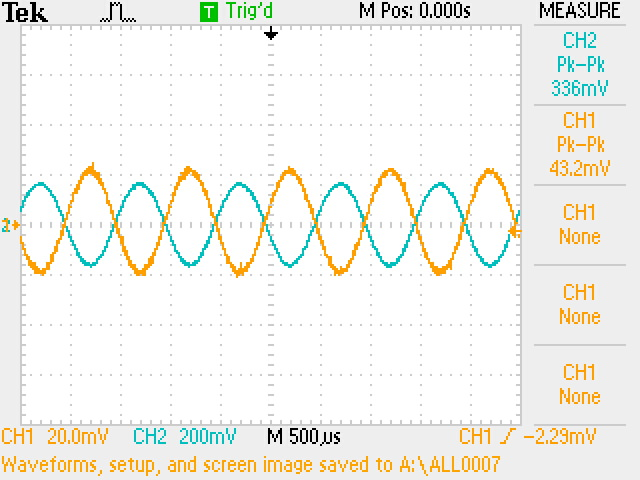
\includegraphics[width = 0.8\textwidth]{scope_8.jpg}}
  \vspace{-8pt}
  \caption{$V_{in}$ (blue) and $V_{out}$ (orange) with $R_{B1}$ and $R_C$ at mid range}
 \end{center}
\end{figure}

It can be seen that for mid range values of  $R_{B1}$ and $R_C$, there is little to no gain in the signal, however there is a phase shift of $180^o$ present on the output due to the capacitor between the collector and $V_{out}$, and the capacitor between $V_{IN}$ and the base.

\begin{figure}[h]
  \vspace{-5pt}
 \begin{center}
  \fbox{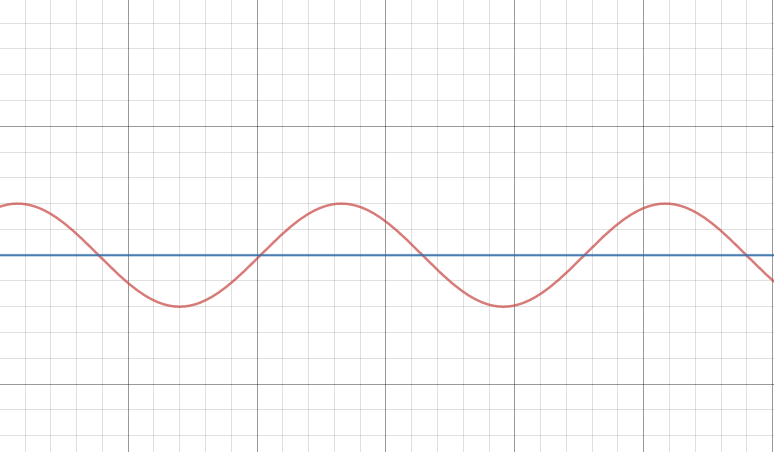
\includegraphics[width = 0.5\textwidth]{0_base.png}
  				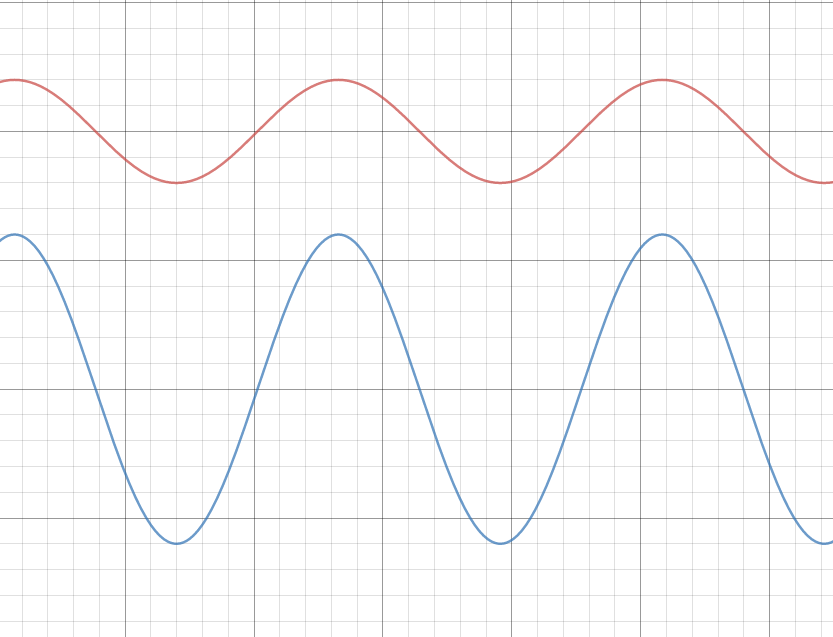
\includegraphics[width = 0.5\textwidth]{1_base.png}}
  \vspace{-24pt}
  \caption{$V_{in}$ (blue) and $V_{out}$ (orange) with $R_{B1}$ and $R_C$ at mid range}
 \end{center}
\end{figure}

Our oscilloscope images for the measurements at points 1 and 2 were not recorded, however figure 5 is what would be expected at these points. When $R_{B1}$ is set to a maximum, there will be no current, and no voltage into point 1 from the DC source, meaning that we will see only the $V_{IN}$ at this point, and seeing as the transistor is not active, there will be 0V on the output. Once we lower $R_{B1}$, there will be a DC voltage applied to the base which will have $V_{IN}$ superimposed upon it. this will then cause the transistor to become active, however the oscillating voltage on $V_B$ will cause it to shift along its voltage current curve, changing how much voltage will be dropped across the transistor. 

\subsection{Voltage gain}

\begin{figure}[h]
  \vspace{-5pt}
 \begin{center}
  \fbox{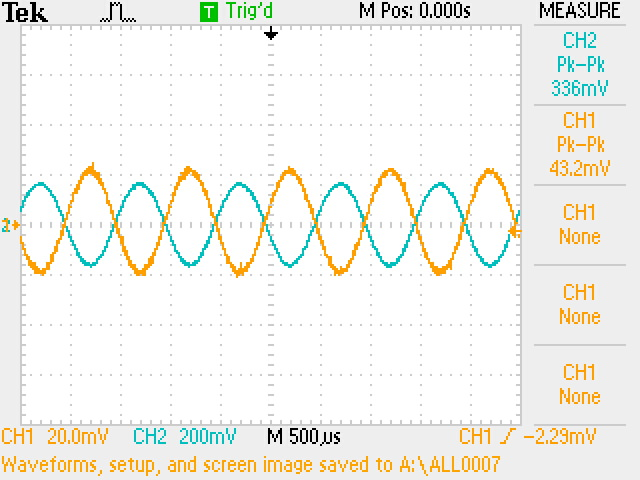
\includegraphics[width = 0.5\textwidth]{scope_8.jpg}
  				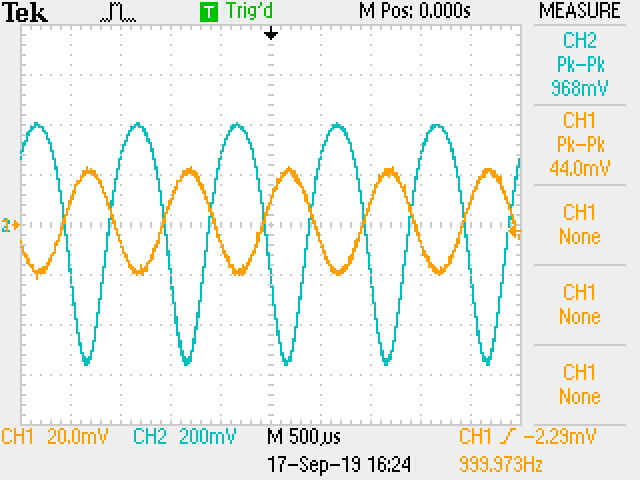
\includegraphics[width = 0.5\textwidth]{scope_7.jpg}}
  \vspace{-24pt}
  \caption{Gain of the transistor}
 \end{center}
\end{figure}

$A = \dfrac{V_o}{V_i}$\\\\
$A_{left} = \dfrac{336}{43.2} = 7.78 $\\\\
$A_{right} = \dfrac{968}{44} = 22 $\\

\subsection{Circuit operation}

The capacitor $C_1$ serves to superimpose the signal  $V_{IN}$ onto whatever DC voltage is allowed into the base by $R_{B1}$. this will then cause the transistor to become active, however the oscillating voltage on $V_B$ will cause the $\beta$ value of the transistor to vary greatly, which will in turn greatly vary what current is allowed through the transistor. This increase and decrease in current will charge and discharge the $C_2$ capacitor from which we are reading $V_{OUT}$. 


 

\pagebreak
\section*{Apendix}
\begin{figure}[h]
 \begin{center}
  \fbox{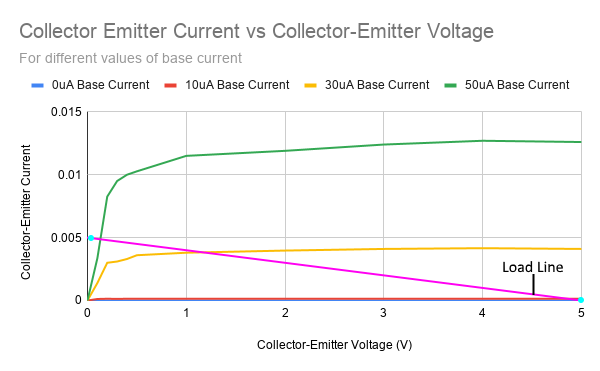
\includegraphics[width = 0.8\textwidth]{load_first.png}}
  \vspace{-10pt}
  \caption{Load line of BJT, with Q-points}
 \end{center}
\end{figure}

\begin{figure}[h]
  \vspace{-15pt}
 \begin{center}
  \fbox{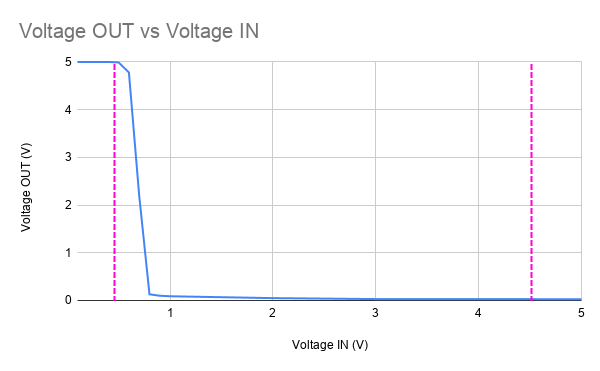
\includegraphics[width=0.8\textwidth]{switch_load.png}}
  \caption{Input-output voltage characteristics of a BJT}
 \end{center}
\end{figure}


\end{document}

